\chapter{Research}\label{research}
%TODO Mention RQ, problem statement
The aim of this thesis is to examine the effect of reducing the dimensionality of the state-space in reinforcement learning (RL). In this section we will discuss our research and its results. We will start by detailing our method in section \ref{research-method}; here we will explain the environments we used for our experiments, as well as the experiments that we ran. After this, we will show and discuss the results from these experiments in section \ref{research-results}. The discussion of the results will include an examination of how the different state-space reduction methods led to their results.

\section{Methodology}\label{research-method}
In this section we will explain our method: how we researched the effect of state-space dimensionality reduction on an RL agent. First, in section \ref{research-exp}, we will explain the experiments in general: the different agent setups that we compared. Then, we will look at the environments in which we ran the experiments in sections \ref{research-env-pysc2} and \ref{research-env-pong}, including their specific agent architectures.

\subsection{Experiments}\label{research-exp}
To examine the effect of the different dimensionality reduction methods, we implemented multiple RL agents using different reduction methods and compared their performance in two environments. In this section we will discuss the agents that we used. We will give a general overview here, and give more details about the architectures of the agents in the sections explaining the used environments: sections \ref{research-env-pysc2} and \ref{research-env-pong}.

The first agent mentioned is the baseline agent, which does not use a dimensionality reduction method, therefore using the full dimensions of the observation received from the environment. All other agents reduce the dimensionality of the observations, thus using less features. The general work flow of these agents is given in figure \ref{fig:rl_cycle_dim}.

\begin{figure}[h]
    \centering
    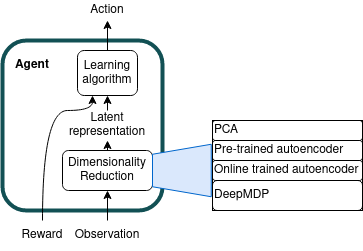
\includegraphics[width=0.45\textwidth]{rl_cycle_dim_red}
    \caption{Overview of the general architecture of an RL agent using a state-space dimensionality reduction method, including the reduction methods used in our experiments. The learning algorithm used is DDQN.}
    \label{fig:rl_cycle_dim}
\end{figure}

Furthermore, to allow for a fair comparison of their performance, all agents must share as many architectural design choices and hyperparameter settings as possible. This is done by extending the baseline agent in all other agents. \par

\noindent \textbf{Baseline agent} \par
\noindent The baseline agent is a standard RL agent that does not use any dimensionality reduction. This is the agent that is extended by all other agents. It uses a DDQN strategy, as explained in section \ref{pl-dqn}. 

An overview of the agent, i.e. a high-level view of DDQN, is given in figure \ref{fig:rl_cycle_base}. First, the agent receives an observation from the environment. This observation is passed to its neural network approximating the Q-function: its policy network. This returns a valuation for each action taken in this state. Then, the agent either chooses the action with the best valuation (i.e. acting greedily) or chooses a random action. Then, the chosen action is performed and we repeat this cycle until the end of the episode, whilst often training the policy network on stored transitions. \par

\begin{figure}[h]
    \centering
    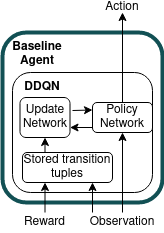
\includegraphics[width=0.2\textwidth]{rl_cycle_baseline_agent}
    \caption{Overview of the baseline agent, using DDQN.}
    \label{fig:rl_cycle_base}
\end{figure}

\noindent \textbf{PCA agent}\par
\noindent The PCA agent uses PCA to reduce the dimensionality of the state observations. As mentioned, this is done by extending the baseline agent: after receiving an observation from the environment, the observation is processed by a PCA component lowering the observation dimensionality. This latent representation is then used by the agent as if it is the actual observations. This means that it is passed to the policy network to give an action valuation, as well as being stored in transitions used to train the network. This is shown in figure \ref{fig:rl_cycle_pca}.

\begin{figure}[h]
    \centering
    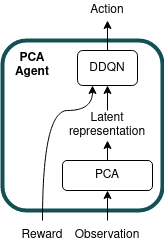
\includegraphics[width=0.2\textwidth]{rl_cycle_pca_agent}
    \caption{Overview of the PCA agent.}
    \label{fig:rl_cycle_pca}
\end{figure}

The PCA component is trained separately before being used by the agent. This is done by training the PCA on previously stored observations, and is agnostic the RL problem. It is important that these observations give a good representation of the entire environment to get a well trained PCA component. \newline \par

\noindent \textbf{Pre-trained autoencoder agent} \par
\noindent This agent is very similar to the PCA agent, except instead of using a PCA component, we are using an autoencoder to reduce dimensionality. Its overview is given in figure \ref{fig:rl_cycle_ae}. Just like the PCA component, the autoencoder is pre-trained on stored observations in an RL problem agnostic manner. After this it is used by the agent to reduce the dimensionality of the observation. 

\begin{figure}[h]
    \centering
    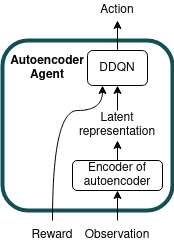
\includegraphics[width=0.2\textwidth]{rl_cycle_autoencoder_agent}
    \caption{Overview of the pre-trained and online trained autoencoder agents.}
    \label{fig:rl_cycle_ae}
\end{figure}

The autoencoder is trained by passing batches of observations to the encoder, which performs the dimensionality reduction. Its output is then passed to the decoder which tries to reconstruct the original data. The loss is then calculated by how similar the decoder output is, compared to the original data. Specifically, the \emph{mean squared error} is used.

When being used by an agent to reduce the dimensionality of an observation, only the encoder part of the autoencoder is used. When we speak of the output of the autoencoder in the context of being used by an agent, we mean the output of the encoder part. The autoencoder is not being trained further while in use by an agent.\newline \par

\noindent \textbf{Online trained autoencoder agent} \par
\noindent  This agent is very similar to the pre-trained autoencoder agent, so we again refer to figure \ref{fig:rl_cycle_ae}. The only difference is the moment of training the autoencoder. In the pre-trained autoencoder agent, the autoencoder is trained before being used by an agent, using previously stored observations. In this online trained autoencoder agent, we are using an autoencoder that has not been pre-trained; it is being trained while being used by the agent. 

In this case, the agent itself still only uses the encoder part of the autoencoder. However, we now also store batches of observations and pass these to the training method of the autoencoder. This training method is the same as before: passing the observations to the encoder, whose output is passed to the decoder, whose output is compared to the original observation to calculate the loss and train the network.\newline\par

\noindent \textbf{DeepMDP agent} \par
\noindent This agent has only been used in the Starcraft II environment, due to time limitations. Just like the online trained autoencoder agent, the DeepMDP agent is completely trained while being used by the agent. It also uses an encoder, which has the same design as the encoders of the autoencoders. Differently from the autoencoder though, this encoder is actually part of the agent's network; whereas the autoencoder is a separate network, the DeepMDP simply extends the network of the agent, thus training the policy network and encoder simultaneously. This is further explained in section \ref{pl-deepmdp}.

In figure \ref{fig:rl_cycle_deepmdp} it can be seen that the observation given by the environment goes directly into the policy network. However, in contrast with the baseline agent, the observation first goes through the encoder, before going into the network representing the Q-function.

\begin{figure}[h]
    \centering
    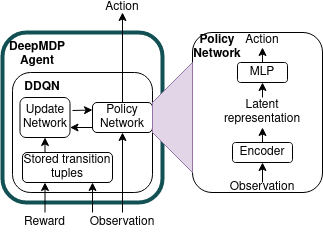
\includegraphics[width=0.5\textwidth]{rl_cycle_deepmdp_agent}
    \caption{Overview of the DeepMDP agent.}
    \label{fig:rl_cycle_deepmdp}
\end{figure}

Another difference with the baseline agent is not shown in the figure: the DeepMDP makes use of an auxiliary objective to calculate the loss while training the policy network: the transition loss. This is also explained in section \ref{pl-deepmdp}.

\subsection{Environment: Starcraft II}\label{research-env-pysc2}
The first environment used for our experiments is the \emph{StarCraft II} environment by \emph{Blizzard}\cite{blizzard}. StarCraft II is a real-time strategy game, which has been used in RL research after the introduction of a learning environment created in collaboration with \emph{DeepMind}, called \emph{SC2LE} and a corresponding Python component called \emph{PySC2}\cite{pysc2}.

In particular we are using a PySC2 minigame called \emph{MoveToBeacon}. This minigame simplifies the StarCraft II game. Here, the RL agent must select an army unit and move it to a given beacon. To simplify our RL agent, selecting the army unit is implemented as a script, thereby focusing our research on moving the army unit to the beacon. A screenshot of the game is given in figure \ref{fig:pysc2_SS}. 

\begin{figure}[h]
    \centering
    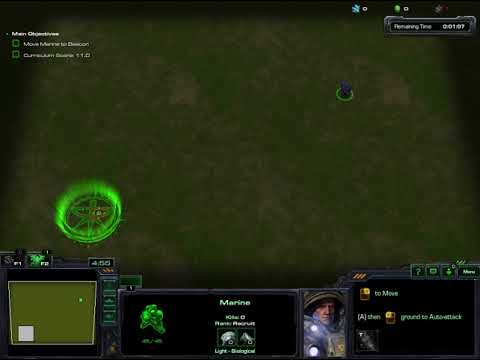
\includegraphics[width=0.45\textwidth]{pysc2_SS}
    \caption{Screenshot of the minigame \emph{MoveToBeacon} in \emph{StarCraft II}.}
    \label{fig:pysc2_SS}
\end{figure}

An \textbf{observation} received by the agent in this minigame is given by a $32 \times 32$ grid, representing the entire state of the game, giving a total of \textbf{$1024$ features}. Each cell in the grid represents a tile in the game. It can have one of three values: a 0 denoting an empty tile, a 1 denoting the army unit controlled by the agent, or a 5 denoting the beacon. The beacon comprises more than one tile, namely a total of $21$ tiles; it comprises five adjecent rows, where the first comprises three adjecent columns, followed by three rows of five columns, followed by a row of three columns, creating a octagonal-like shape. Because of this, the beacon has $27 \cdot 27$ places where it could be, with the army unit having $1003$ tiles left to be. This gives a total state-space of $27 \cdot 27 \cdot 1003 = 731.187$. An example of such a state observation can be seen in figure \ref{fig:state_example}.

\begin{figure}[h]
    \centering
    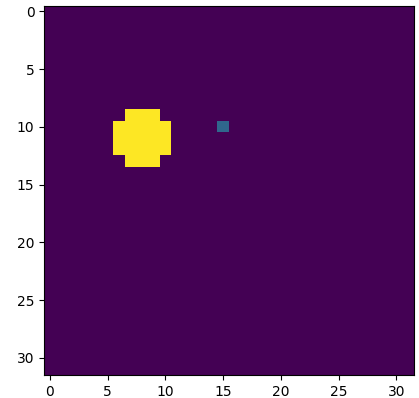
\includegraphics[width=0.35\textwidth]{AE_State_original}
    \caption{A state observation received by the RL agent, for the StarCraft II minigame MoveToBeacon. The yellow cells represent one beacon; the blue cell represents the army unit controlled by the player; all other cells are empty.}
    \label{fig:state_example}
\end{figure}

An \textbf{action} taken by the agent is given by an $(x,y)$ coordinate with $x,y \in \{0 .. 31\}$. This denotes the (indices of the) cell in the grid that the army unit will move to. Each action sent to the environment will result in $8$ in-game steps, meaning that if the given coordinates are further away than 8 steps, the unit will only walk 8 steps towards the given coordinates before the agent has to choose a new action.

Lastly, an \textbf{episode} takes $120$ seconds. The goal is to move the army unit to the beacon as often as possible in this time limit, each time adding $1$ point to the episode score. At the start of each episode, the beacon and army unit are placed randomly. Whenever the army unit reaches the beacon, only the beacon will be relocated randomly. 

Within the $120$s time limit, the agent will be able to take 239 steps/actions. An agent following a random policy gets a score of about $0-3$ points per episode (again, one point for each time the army unit reaches the beacon), whereas a scripted agent scores about $25-30$ points per episode (meaning the agent on average needs $8$ or $9$ actions before reaching a beacon).

\subsubsection*{Agents setup}
We will now explain the architectures of the agents used in the Starcraft II environment. We will only give a general overview, referring to appendix \ref{appendix} section \ref{appendix-agents} for details on the neural network architectures and hyperparameter settings. 

Whereas the baseline agent uses the $32 \times 32$ observations given by the environment, all other agents reduce the dimensionality to $16 \times 16$. This means that the number of features in an observation are reduced from $1024$ to $256$.

Though the baseline agent's architecture is extended by all other agents (in order to keep the agents as similar as possible), one important change must be made. The policy networks of all agents are convolutional neural networks, and the output dimensions of a convolutional layer depends on the dimensions of its input. The baseline agent's policy network receives a $32 \times 32$ input, whereas the other agents receive a $16 \times 16$ input. In all cases, the output dimensions must be $32 \times 32$. This is because the network approximates the Q-function: a valuation of all actions for a given state. Since an action in our environment is defined by the coordinates the army unit must walk to, there are $32 \times 32$ possible actions. To deal with this difference in input dimensions, the first layer of the policy networks of the non-baseline agents are modified (using different stride and padding sizes) to increase the output dimensionality to $32 \times 32$.\newline\par

\noindent \textbf{Baseline agent}\par
\noindent The baseline agent is a standard RL agent that does not use any dimensionality reduction and is extended by the other agents.

Its policy network consists of three convolutional layers: the first layer being a transposed convolutional layer \cite{transpose}, the other two being regular convolutional layers. The use of the transposed convolutional layer allows for the possibility of upsampling the dimensionality of the given input. This is needed in agents using dimensionality reduction, where the input for the network is $16 \times 16$, but the output needs to be $32 \times 32$ to cover the action space. However, for our baseline agent, the input dimensions, $32 \times 32$, must remain the same, which is achieved by setting the stride of the first layer to $1$. This way, both the dimensions of the input and the output of the network are $32 \times 32$ (where its input represents the current state observation and its output the action valuations).\newline\par

\noindent \textbf{PCA agent}\par
\noindent The PCA agent uses PCA to reduce the dimensionality of the state observations from $32 \times 32$ to $16 \times 16$. To do this, the observation input must first be flattened, and the output of the PCA must be reshaped to $16 \times 16$.

The output of the policy network representing the Q-function must remain $32 \times 32$, since we have $32 \cdot 32$ possible actions: one action per coordinate. Therefore, the first layer in the policy network, the aforementioned transposed convolutional layer, has a stride of $2$ and an output padding of $1$. This changes the dimensions from $16 \times 16$ to $32 \times 32$. 

The PCA component is trained on $240.000$ previously stored observations, which corresponds to observations from $1000$ episodes. These have been gathered using a scripted agent. The first $256$ principal components in our PCA (representing a $16 \times 16$ dimensional observation), contain roughly $96\%$ of the variance of the original data. We are using a scalar to standardize the observation data as explained in section \ref{pl-pca}. \newline\par

\noindent \textbf{Pre-trained autoencoder agent}\par
\noindent Just like the PCA component, the autoencoder is pre-trained on the same $240.000$ observations. After this its encoder is used by the agent to reduce the dimensionality of the observation. 

The encoder and decoder of the autoencoder are convolutional neural networks. The encoder uses two convolutional layers: the first has a stride of $2$, which reduces the dimension to $16 \times 16$. The decoder, which tries to reconstruct the original data, uses three convolutional layers. The first layer is a transposed convolutional layer with a stride of $2$, to bring the dimensions back to $32 \times 32$. The other two layers are regular convolutional layers. \newline\par
 
\noindent \textbf{Online trained autoencoder agent} \par
\noindent  This agent has the exact same design as the pre-trained autoencoder agent. As mentioned, the only difference is the moment of training the autoencoder: instead of training on previously stored observations, we are now training the autoencoder simultaneously with the RL agent. \newline\par

\noindent \textbf{DeepMDP agent}\par
\noindent The encoder of the DeepMDP has the same design as the encoders of the autoencoders: one convolutional layer with stride $2$ to reduce dimensions and a second convolutional layer with stride $1$. 

The auxiliary objective to calculate the transition loss represents the cost of all possible transitions from a given latent representation. This means that its output has dimensions $(32 \cdot 32) \times 16 \times 16$. The tuple $(32, 32)$ represents the actions that can be taken in the current state, while the other two dimensions, $16 \times 16$ represent the next (predicted) latent observation. It has only one layer, a convolutional layer, with $32 \cdot 32$ output channels to represent the action dimensions.

\subsection{Environment: OpenAI Pong}\label{research-env-pong}
The second environment in which we ran our experiments is the Atari game Pong, using the OpenAI Gym environment \cite{pong}. In figure \ref{fig:pong-screen}, a screenshot of the game is given. In the game, two players try to score points by getting a ball behind the opponent. Both players control one paddle that can be moved vertically, to bounce to ball off of. The first player to score $21$ points wins.

\begin{figure}[h]
    \centering
    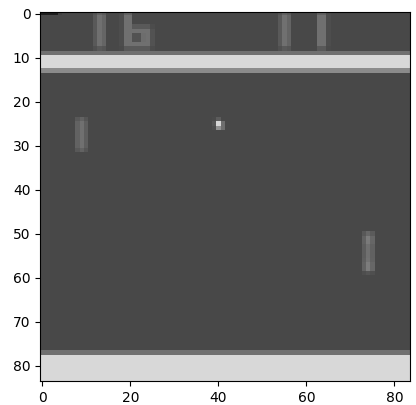
\includegraphics[width=0.25\textwidth]{Pong/Frame}
    \caption{A screenshot from the OpenAI Gym Atari game Pong.}
    \label{fig:pong-screen}
\end{figure}

\emph{Observations} are created from frames of the game: screenshots containing pixel values. Each frame is processed to a $84 \times 84$ grayscaled image. To capture movement in an observation, each observation consists of four consecutive frames. This is shown in figure \ref{fig:pong-obs}. This is done by stacking the four frames, thereby creating $4$ colour channels for a CNN input. Since each step in the game gives a single new frame, each observation only has one of its four frames different from the previous observation.

\begin{figure}[h]
    \centering
    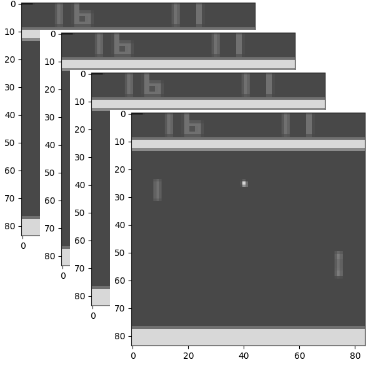
\includegraphics[width=0.2\textwidth]{Pong/Observation}
    \caption{A single observation in OpenAI Gym's Pong: four consecutive stacked frames.}
    \label{fig:pong-obs}
\end{figure}

An $84 \times 84$ frame means there are $ 84 \cdot 84 = 7056$ features per frame (thus for a single observation consisting of four frames, this would total to $84 \cdot 84 \cdot 4 = 28224$ features). Both paddles can move up and down to $64$ spaces, giving $64 \cdot 64$ possible states when only looking at the paddle placement. Furthermore, the ball can be in any place in the $64 \times 84$ playing field. This gives a total state-space of $(64 \cdot 64) \cdot (64 \cdot 84) = 22020096$. 

The agent, controlling one paddle, has six possible \emph{actions} it can take. Most important are the actions \textit{right} and \textit{left}, moving the paddle up and down respectively. Another relevant action is \textit{noop}, to not move the paddle. Other actions include an action to start the game (\textit{fire}) and actions used for other Atari games, but meaningless in Pong (\textit{rightfire} and \textit{leftfire}). 

An \emph{episode} ends when one player reaches $21$ points. After each step, the agent either receives a reward of $1$ if it scored a point, $-1$ if the opponent scored a point, or $0$ otherwise. At the end of the episode, the final score of the agent is calculated as the difference between its own and the opponent's points (e.g. a final score of $2$ means it won the game $21 - 19$). Thus, a perfect score would be $21$. A random agent mostly scores between $-21$ and $-18$.

\subsubsection*{Agents setup}
The same agents are used for experiments in this environment as in the Starcraft II environment, excluding the DeepMDP agent due to time limitations. Again, we only give a general overview of the agents' architectures, referring to appendix \ref{appendix} section \ref{appendix-agents-pong} for more details.

The baseline agent receives a $4 \times 84 \times 84$ state observation input: four consecutive $84 \times 84$ stacked frames. This totals to $28224$ features per observation. All state-space dimensionality reduction methods, project a single $84 \times 84$ frame down to $42 \times 42$, thus reducing the number of features down from $7056$ to $1764$. Thus, agents using a dimensionality reduction method, receive a $4 \times 42 \times 42$ state observation, totaling to $7056$ features per observation. \newline\par

\noindent \textbf{Baseline agent}\par
\noindent The baseline agent is a standard DDQN RL agent that does not use any dimensionality reduction and is extended by the other agents.

Its policy network, representing the Q-function, consists of three convolutional layers and two linear layers. The first conv layer has a kernel size of $6$ and a stride of $3$, the second conv layer a kernel size of $4$ and stride of $2$, and the final conv layer a kernel size of $3$ and stride of $1$. These settings affect the output shape of each layer. For this, the $4$ colour channels are irrelevant. Looking at a single colour channel, its $84 \times 84$ input is first downsampled to $27 \times 27$, then to $12 \times 12$ and finally to $10 \times 10$. The final conv layer's output is flattened before going into the first linear layer. The final linear layer has an output of $6$, corresponding to the action-space.\newline\par

\noindent \textbf{PCA agent}\par
\noindent The PCA agent uses PCA to reduce the dimensionality of a single frame from $84 \times 84$ to $42 \times 42$. To do this, the observation input must first be flattened, and its output must be reshaped to $42 \times 42$. The final observation shape is thus $4 \times 42 \times 42$.

The policy network, representing the Q-function, is identical to the baseline agent. Now that we have a $42 \times 42$ input per colour channel, the convolutional layers in the policy network downsample the input first to $13 \times 13$, then to $5 \times 5$ and finally to $3 \times 3$.

The PCA component is trained on $40.000$ previously stored frames, which corresponds to roughly $40$ episodes, but were taken randomly across $300$ episodes. These have been gathered using the baseline agent. The first $1764$ principal components in our PCA (representing a $42 \times 42$ dimensional observation), capture roughly $99\%$ of the variance of the original data. Since we are already using (gray)scaled data, we do not use a scalar for the PCA  as mentioned in \ref{pl-pca}. \newline\par

\noindent \textbf{Pre-trained autoencoder agent}\par
\noindent The autoencoder is pre-trained on $925.000$ frames, taken from $600$ episodes. After this its encoder is used by the agent to reduce the dimensionality of a single frame. This, like the PCA agent, results in a observation of $4 \times 42 \times 42$.

The encoder and decoder of the autoencoder are convolutional neural networks. The encoder uses three convolutional layers: the first has a stride of $2$, which reduces the dimensions to $42 \times 42$. The decoder, which tries to reconstruct the original data, uses two convolutional layers. The first layer is a transposed convolutional layer with a stride of $2$, to bring the dimensions back to $84 \times 84$. The second layer is a regular convolutional layer. \newline\par
 
\noindent \textbf{Online trained autoencoder agent}\par
\noindent  This agent has the exact same design as the pre-trained autoencoder agent. As mentioned, the only difference is the moment of training the autoencoder: instead of training on previously stored observations, we are now training the autoencoder simultaneously with the RL agent.

\subsection{Remarks on dimensionality reduction methods}
There are two methods we would like to shortly mention that we did not use in our experiments. Firstly, another popular method to reduce dimensionality of data is \emph{t-distributed stochastic neighbor embedding} (t-SNE) \cite{tsne}. Though widely used to reduce the dimensionality of data, it is unsuitable for our purposes. This has to do with the way t-SNE works. To calculate the data points in the lower dimensional space, it first calculates the Euclidean distance between all data points, which is transformed to a probability distribution. From this it follows that the data projection to a lower dimensional space is inherently dependent on the input data. In other words, we cannot train t-SNE on training data and then apply its transformation on new data. This makes it unusable for us, since we need to be able to transform a single observation (and therefore need to be able to separate the training process and the transformation process). 

A second method we did not use in our experiments is \emph{Max-pooling}. Max-pooling is a type of layer in a CNN that downsamples its input. However, compared to using a convolutional layer with a stride of $2$ as used in our experiments, "when pooling is replaced by an additional convolution layer with stride $r = 2$ performance stabilizes and even improves on the base model" \cite{maxvsconv}.
 

\section{Results}\label{research-results}
In this section we will show and discuss the results from the experiments mentioned in section \ref{research-exp}. We will start by showing the results from the Starcraft II environment in section \ref{research-results-pysc2}, before showing the results of the OpenAI Pong environment in section \ref{research-results-pong}. These sections will focus on the research sub-questions: how do the training results of a double deep-Q-network reinforcement learning agent change when using PCA, autoencoders and DeepMDPs for state-space dimensionality reduction in Starcraft II MoveToBeacon and OpenAI Atari Pong? They will also include a discussion of the results and an examination of how the different state-space reduction methods led to their results. In section \ref{research-discussion} we will give a general discussion of all results to answer the main research question: what is the effect of state-space dimensionality reduction on model-free value-based reinforcement learning in an environment using grid-based observations, by using PCA, autoencoders or DeepMDPs?

\subsection{Research results: Starcraft II}\label{research-results-pysc2}
\subsubsection{Results overview}
The results from running the different agents in the Starcraft II minigame MoveToBeacon, can be seen in figure \ref{fig:results-agents}. For each agent, the score, i.e. return, per episode is shown, as well as an average score per $30$ episodes. Again, a scripted agent scores around $25-30$ per episode, and an agent following a random policy around $0-3$.


\begin{figure}[h!]
	\centering
	\begin{subfigure}[b]{0.45\textwidth}
		\includegraphics[width=\linewidth]{Base_agent_results}
		\caption{Results for the baseline agent.}
		\label{fig:results-base} 
	\end{subfigure}\hfill
	\begin{subfigure}[b]{0.45\textwidth}
		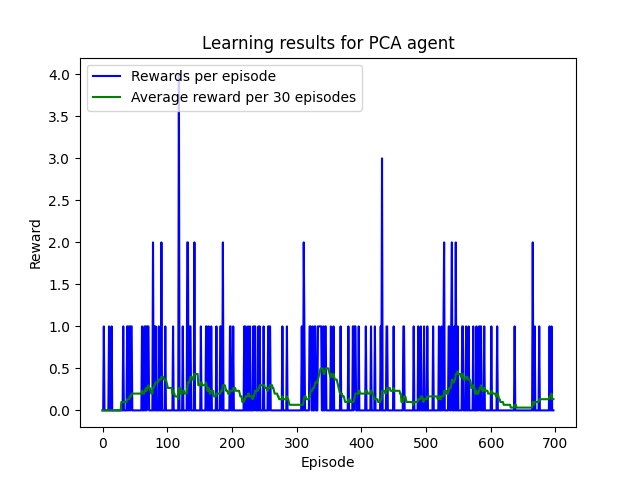
\includegraphics[width=\linewidth]{PCA_with_scalar_agent_results}
		\caption{Results for the PCA agent.}
		\label{fig:results-pca}
	\end{subfigure}
	
	\medskip
	\begin{subfigure}[b]{0.45\textwidth}
		\includegraphics[width=\linewidth]{Pretrained_autoencoder_agent_results}
		\caption{Results for the pre-trained autoencoder agent.}
		\label{fig:results-ae}
	\end{subfigure} \hfill
	\begin{subfigure}[b]{0.45\textwidth}
		\includegraphics[width=\linewidth]{Online_autoencoder_agent_results}
		\caption{Results for the online trained autoencoder agent.}
		\label{fig:results-online-ae}
	\end{subfigure}
	
	\medskip
	\begin{subfigure}[b]{0.45\textwidth}
		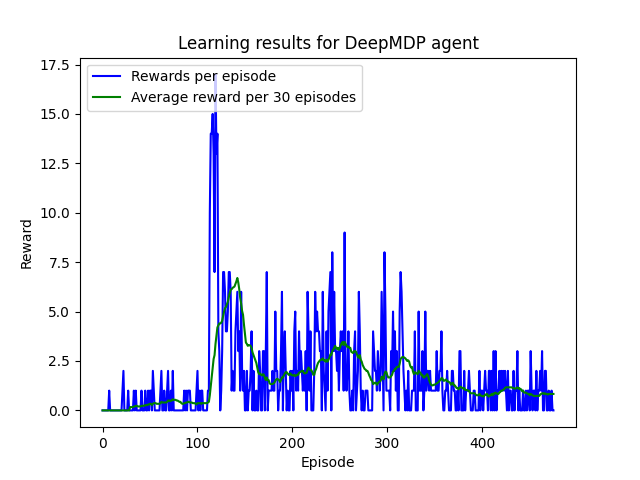
\includegraphics[width=\linewidth]{Deepmdp_agent_results}
		\caption{Results for the DeepMDP agent.}
		\label{fig:results-deepmdp}
	\end{subfigure}
	\caption{Results of the different RL agents in Starcraft II.}
	\label{fig:results-agents}
\end{figure}

As can be seen in subfigure \ref{fig:results-base}, the baseline agent converges to a policy scoring around $19$ per episode. This policy is reached after roughly $600$ episodes. Already after episode $300$ does it oscillate around scoring $17-20$ while also sometimes having an episode score of around $10$. After this it still needs another $300$ episodes to get to a more consistent policy.

The results for the PCA agent can be seen in figure \ref{fig:results-pca}. No matter what neural network architecture used in the agent (having used multiple different linear network architectures and different CNN architectures), it always remained at a policy performing at the level of a random policy, i.e. scoring around $0-3$ per episode.

The results for the agent using a pre-trained autoencoder, in figure \ref{fig:results-ae}, show that this agent performs a little better than the baseline agent. Not only does it converge to a slightly better policy scoring around $21$ per episode, it also converges quicker; it is already consistent after roughly $400$ episodes, instead of $600$. 

Compared to the pre-trained autoencoder agent, the agent using an untrained autoencoder that is being trained while the agent is trained, performs a little worse. It converges after roughly $500$ episodes to a policy around $19-21$. Not only does it take longer to converge and converges to a slightly worse policy, it is also less consistent. Even after $400$ it still has episodes scoring around $13$. This shows it is less consistent than its pre-trained counterpart. However, it still matched the performance of the baseline agent.

Lastly we have the DeepMDP agent. After $130$ episodes, this agent suddenly jumps up from a random policy to scoring around $15$. However, after several episodes it starts going back down, alternating between scoring at a random policy and scoring around $7$, until finally reaching a random policy again. 

Furthermore the training times per episode for each agent were very similar, except for the DeepMDP agent. For all agents but the DeepMDP agent, each episode took only a few seconds with a total training time of roughly $1.5$ hours for $1000$ episodes, whereas each episode in the DeepMDP agent takes $2.5$ minutes. The time to pass an observation through a PCA component or an autoencoder is negligible; the total training times for PCA agent and pre-trained autoencoder agent were almost identical to the baseline agent. Pre-training the PCA or the autoencoder on $1000$ episodes worth of observations only took $3$ minutes ($0.003$ minutes per episode). For the online trained autoencoder agent this means an additional $3$ minutes of training time; approximately a $3.3\%$ increase.

\subsubsection{Discussion}\label{research-discussion-pysc2}
\paragraph{PCA Agent: losing all spatial information}
The first notable result is the PCA agent giving a policy that remains at the level of a random policy during its $800$ episode training, therewith performing way worse than the other agents. A possible explanation might be that the PCA reduction loses (too much) spatial information. Although PCA can be used for image compression, where spatial information is retained, it is a more lossy than an autoencoder \cite{pca_ae}.

Figure \ref{fig:pca-state} shows an example of the PCA transformation on an observation. Figure \ref{fig:pca-original} shows the original observation that the agent would get from the environment. Figure \ref{fig:pca-latent} shows the latent representation after using PCA for dimensionality reduction. As mentioned before, this uses $256$ principal components, capturing roughly $96\%$ of the original data. Here we can see that no spatial information is retained, making it impossible for the agent to train a meaningful policy on. 

Furthermore, we also tested a different PCA setup where we used all $1024$ principal components. Here, we again fitted the PCA on the same observations but keeping all principal components, giving a new $32 \times 32$ observation (and therefore not doing any dimensionality reduction). Transformation of an observation gave similar results: spatial information was lost. The problem therefore lies in the fitting process. A possible explanation for the bad transformation performance, might be that a single observation is very sparse. Even though the PCA is fitted on $240.000$ observations, each single observation is very sparse and at the same time there are a lot of different possible observations due to the large state-space (see section \ref{research-env-pysc2}). This combination might lead to the PCA not being able to generalize well enough.

\begin{figure}[h!]
	\centering
	\begin{subfigure}[b]{0.3\textwidth}
		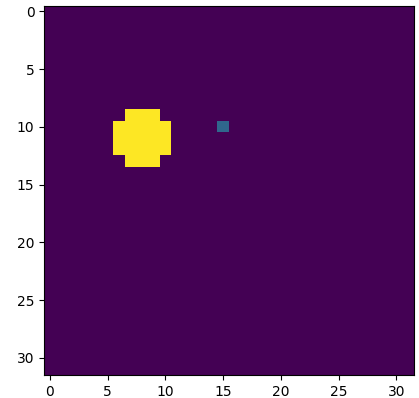
\includegraphics[width=\linewidth]{AE_State_original}
		\caption{The original observation, i.e. the input for the PCA transformation.}
		\label{fig:pca-original} 
	\end{subfigure}\hfill
	\begin{subfigure}[b]{0.3\textwidth}
	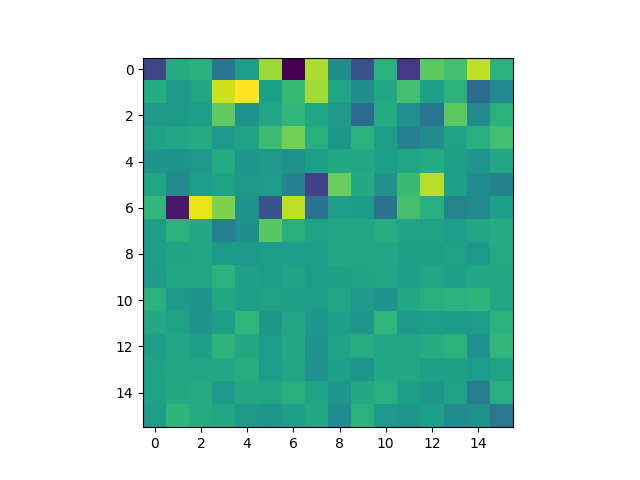
\includegraphics[width=\linewidth]{pca_with_scalar_latent_state}
		\caption{The latent representation given by the PCA transformation}
		\label{fig:pca-latent}
	\end{subfigure}
	\caption{Latent representation of a state observation using PCA in Starcraft II.}
	\label{fig:pca-state}
\end{figure}

\paragraph{Autoencoder agents analyses: outperforming baseline agent}
Another interesting result is the performance of the pre-trained autoencoder agent. Not only does it match the baseline agent's performance, it even slightly surpasses it: it finds a slightly better policy (scoring around $21$ per episode on average, versus $19$), and more quickly converges to a consistent policy (after $400$ episodes versus $600$). Its better performance is despite the agent using imperfect information, while the baseline agent uses complete information.

Its performance is highly dependent on the quality of the output of the autoencoder, which is corroborated in the discussion of the experiments in the second environment, Pong \ref{research-discussion-pong}. To get an understanding of why this agent achieves such good results, we will now examine the autoencoder in detail. We first show the results of training the autoencoder itself. As mentioned, it is trained on $240.000$ observations, corresponding to $1000$ episodes. Whereas each agent's training (except for the DeepMDP) took roughly $90$ minutes, training the autoencoder itself on $1000$ episodes worth of observations only took about $2.5$ minutes. The loss history for the autoencoder can be seen in figure \ref{fig:ae-loss}. After roughly $6000 \cdot 25 = 150.000$ observation it converges to its final loss.

\begin{figure}[h!]
    \centering
    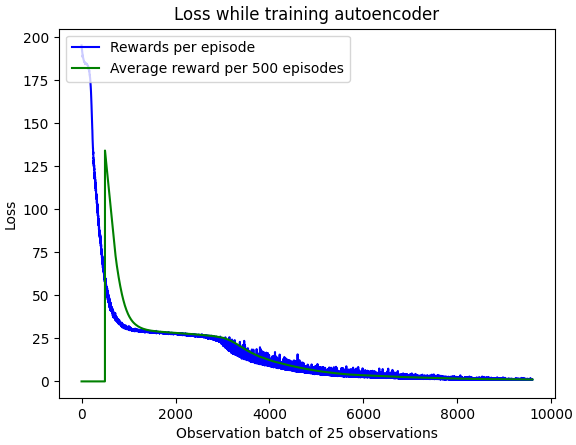
\includegraphics[width=0.5\textwidth]{ae_loss}
    \caption{Losses per 25 observations for training the autoencoder on $240.000$ state observations.}
    \label{fig:ae-loss}
\end{figure}

To analyse the autoencoder, we show the latent representation of the autoencoder (given by the encoder) in figure \ref{fig:ae-featuremap}. The original $32 \times 32$ input for the encoder is given in figure \ref{fig:ae-featuremap-original}. Like before, the yellow octagon is the beacon, the blue square is the army unit controlled by the agent, and purple parts are the empty tiles. The latent representation is given in figure \ref{fig:ae-featuremap-layer2}. Here we can see that the autoencoder compresses the observation down to a similar but smaller observation: each latent cell seems to represent a block of cells of the original data. 

Such a projection onto a lower dimensional space, could create problems for the agent where high precision is involved, since the latent representation will lose at least some of the spatial information. However, in a setting like this, such lack of precision is not important due to the beacon encompassing several pixels. The agent only needs to reach some part of this beacon, thus there is room for locational variance. 

\begin{figure}[h!]
	\centering
	\begin{subfigure}[b]{0.30\textwidth}
		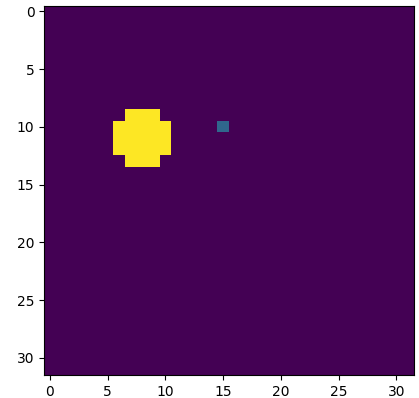
\includegraphics[width=\linewidth]{AE_State_original}
		\caption{The original observation, i.e. the input for the autoencoder.}
		\label{fig:ae-featuremap-original} 
	\end{subfigure}\hfill
	\begin{subfigure}[b]{0.30\textwidth}
		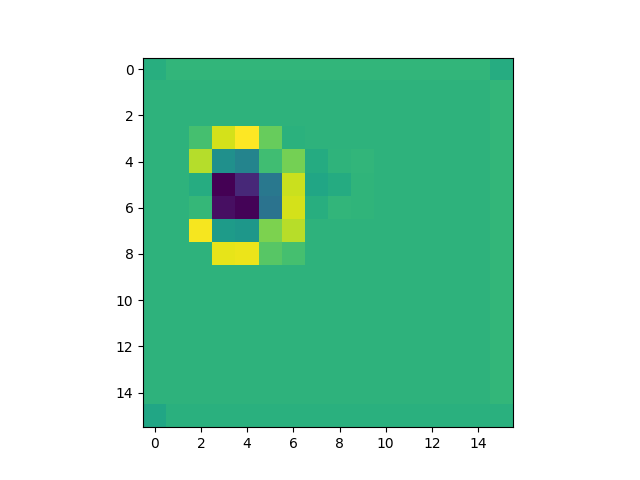
\includegraphics[width=\linewidth]{AE_Layer_2_Feature_Map}
		\caption{The latent representation of the autoencoder, i.e. the output of the encoder.}
		\label{fig:ae-featuremap-layer2}
	\end{subfigure}
	\caption{The latent representation of the autoencoder.}
	\label{fig:ae-featuremap}
\end{figure}

To analyse the autoencoder further, a correlation matrix is given in figure \ref{fig:ae-corr}. Based on $60.000$ state observations, it shows the correlation between the features of the original state observations (i.e. the input for the autoencoder) and the reduced state observations (i.e. the output of the autoencoder). The process of creating this matrix is shown in figure \ref{fig:ae-corr-process}. The original data has dimensions of $32 \times 32$, whereas the reduced data has dimensions of $16 \times 16$, resulting in $1024$ and $246$ features respectively. The $256$ latent features are shown on the x-axis, and the $1024$ original features are shown on the y-axis in figure \ref{fig:ae-corr}. Dark/black and light/beige colouring mean a high correlation (negative and positive correlation respectively), whereas a red colouring means no correlation and the white space means there was too little variance to calculate a correlation. The latter case simply follows from the beacon and army unit not visiting these parts of the map enough times during the used episode observations, which results in too little variance for a correlation to be calculated.

\begin{figure}[h]
	\centering
	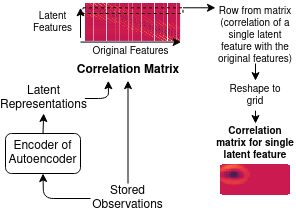
\includegraphics[width=0.4\paperwidth]{Corr_matrix_method}
	\caption{Process of creating a correlation matrix for the latent features with the original features, and creating the correlation matrix of a single latent feature with the original features.}
	\label{fig:ae-corr-process}
\end{figure}

What can be seen from this matrix, is that each cell in the reduced data grid, correlates to a block (a few adjacent rows and columns) of cells of the original data grid. This explanation can be abducted from each feature of the reduced data being highly correlated to a few features of the original data, then being uncorrelated for $32$ features, after which highly correlated features are found again. This jump of $32$ features corresponds to a jump of one row in the original data grid. Thus, a reduced feature correlates to a block of the original features.

This is better visualised by taking the correlation matrix of a single latent feature. The process of this is also shown in figure \ref{fig:ae-corr-process}. We choose a latent feature and take the correlation results of that feature from the correlation matrix, simply by taking the corresponding column from the matrix. We now have the correlation data of a single latent feature with all original features. We then reshape this data to a $32 \times 32$ shape for visualisation. In figure \ref{fig:latent-feature-corr} we have done this for latent feature $68$. In subfigure \ref{fig:ae-latent-feature} we can see where latent feature $68$ lies in the $16 \times 16$ latent space: in the 4th column of the 4th row. In subfigure \ref{fig:ae-latent-feature-corr-matrix} the correlation matrix for this latent feature with all original features is shown.

Here we can see clearly the high correlation of the latent feature with a octagonal shape of original features. This relates to the octagonal shape of the beacon, the most dominant part of the observation. Thus, the autoencoder is taking in the values of a roughly $14$ by $14$ octagonal shape of pixels to get the value for a latent feature, thereby compressing the image to a lower dimension.

This autoencoder agent not only outperforms the baseline agent, it also outperforms the online trained autoencoder agent. This latter agent converges to a slightly worse policy and takes more episodes to converge, while remaining not very consistent (sometimes scoring only about $13$ points in an episode). This can be explained by the fact that this agent not only trains a policy network, but also, separately, the autoencoder. This means that for many episodes, the policy network is trained on a rather imperfect representation; the pre-trained autoencoder needed roughly $150.000$ observations before getting close to its final loss. Still, it got to a policy similar to the baseline agent (even scoring slightly better on average) in a similar number of episodes; the main difference being that the baseline agent is much more consistent.

Besides outperforming the online trained autoencoder agent, the pre-trained agent has another advantage. Since the autoencoder can be trained separately from the agent, we can reuse the autoencoder for different agents acting in the same environment but solving a different RL problem. This allows for the possibility of training an autoencoder once, after which different agents can be trained on less features, allowing for less computation cost to train each agent. This is also substantiated by the autoencoder taking comparatively little time to train.


\begin{figure}[h]
	\centering
	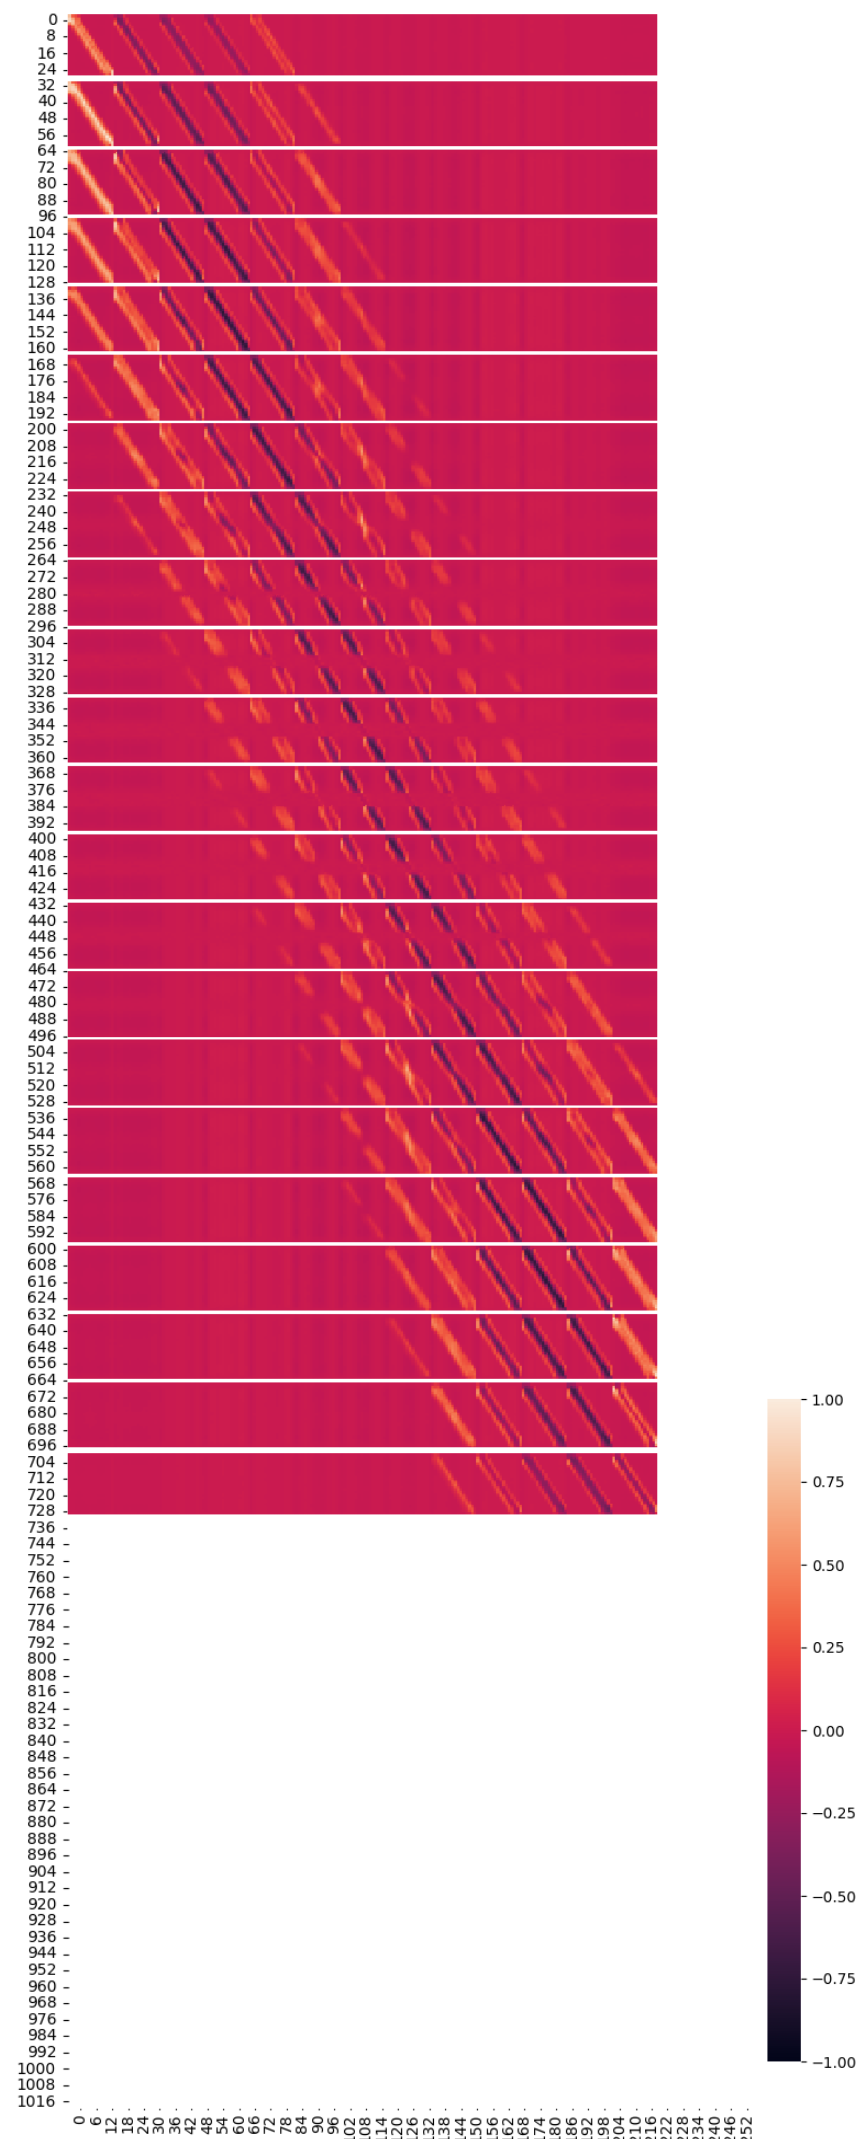
\includegraphics[width=0.35\paperwidth]{AE_corr_matrix_cropped}
	\caption{Correlation matrix for the autoencoder used in the pre-trained autoencoder agent, based on $60.000$ state observations. The x-axis contains the features of the reduced state observations, and the y-axis contains the features of the original observations.}
	\label{fig:ae-corr}
\end{figure}

\begin{figure}[h]
	\centering
	\begin{subfigure}[b]{0.2\textwidth}
		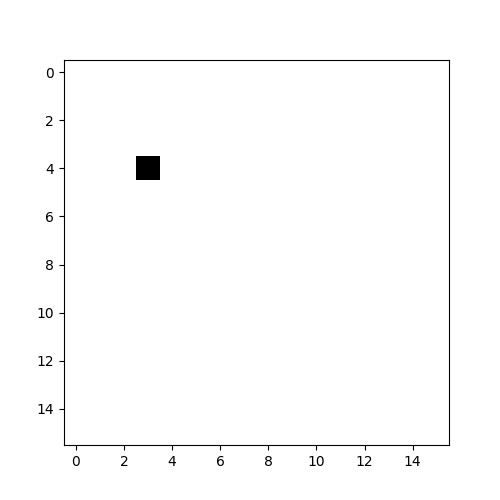
\includegraphics[width=\linewidth]{Grid_latent_feature_68}
		\caption{The latent feature that was used: at index $67$ of flattened grid data.}
		\label{fig:ae-latent-feature} 
	\end{subfigure}\hfill
	\begin{subfigure}[b]{0.75\textwidth}
		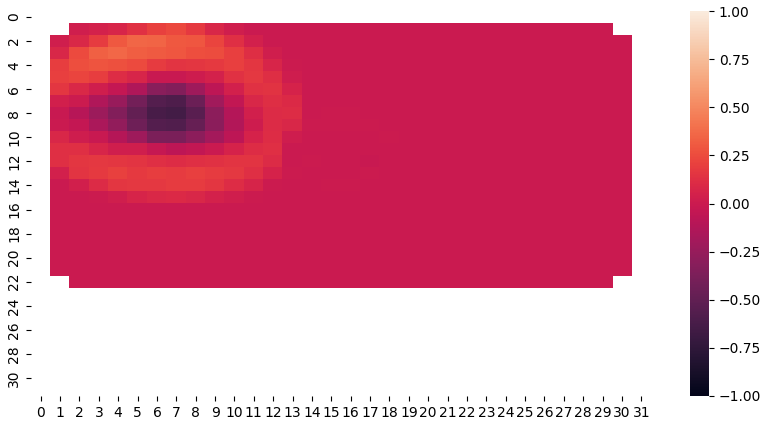
\includegraphics[width=\linewidth]{corr_matrix_latent_feature_68}
		\caption{Correlation matrix for latent feature $68$ with the original features.}
		\label{fig:ae-latent-feature-corr-matrix}
	\end{subfigure}
	\caption{The correlation matrix for latent feature $68$ with the original features.}
	\label{fig:latent-feature-corr}
\end{figure}

\paragraph{DeepMDP agent: unable to balance multiple loss calculations}

Lastly, the DeepMDP agent is unable to converge. After roughly $120$ episodes, it gets to a decent policy, scoring around $15$ per episode. Quickly after though, it drops down to scoring between $0$ and $10$, before dropping further down after $400$ episode to scoring between $0$ and $5$, only slightly better than a random policy.

The DeepMDP agent seems to have trouble with balancing the multiple losses being calculated; a recurring problem that is also described in the paper introducing DeepMDPs \cite{deepmdp}. When after approximately $130$ episodes the score falls from roughly $15$ down to around $5$, the total loss being calculated decreases significantly. However, it is only the gradient penalty for the auxiliary objective, i.e. the gradient penalty for the transition cost network, that has a lower loss value.  All other losses, i.e. the remaining gradient penalties, the transition cost and the DDQN loss, are all increased. Most notably the DDQN loss is increased, resulting in a worse Q-function network, thus giving lower scores.

This trouble with balancing the loss is further demonstrated at $240$ episodes into training. At this moment, the DDQN loss, as well as the gradient penalties for the Q-function and encoder networks, are all decreasing in value. This results in higher average episode scores. However, after this they start increasing again, leading to a further drop in episode scores around $330$ episodes.

\clearpage
\subsection{Research results: OpenAI Pong}\label{research-results-pong}
\subsubsection{Results overview}
The results for the different RL agents in OpenAI Pong can be seen in figure \ref{fig:results-agents-pong}. As with Starcraft II, each agent's score is shown per episode, as well as a $30$ episode average. A perfect agent would score $21$ points per episode, whereas a random agent will score mostly between $-21$ and $-18$.

\begin{figure}[h]
	\centering
	\begin{subfigure}[b]{0.49\textwidth}
		\includegraphics[width=\linewidth]{Pong/Base_agent_results}
		\caption{Results for the baseline agent.}
		\label{fig:results-base-pong} 
	\end{subfigure}
	\begin{subfigure}[b]{0.49\textwidth}
		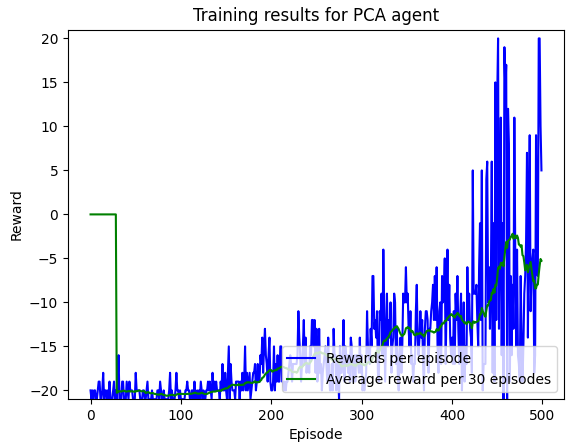
\includegraphics[width=\linewidth]{Pong/PCA_agent_results}
		\caption{Results for the PCA agent.}
		\label{fig:results-pca-pong}
	\end{subfigure}
	
	\medskip
	\begin{subfigure}[b]{0.49\textwidth}
		\includegraphics[width=\linewidth]{Pong/Pretrained_autoencoder_agent_results}
		\caption{Results for the pre-trained autoencoder agent.}
		\label{fig:results-ae-pong}
	\end{subfigure}	
	\begin{subfigure}[b]{0.49\textwidth}
		\includegraphics[width=\linewidth]{Pong/Online_autoencoder_agent_results}
		\caption{Results for the online trained autoencoder agent.}
		\label{fig:results-online-ae-pong}
	\end{subfigure}
	\caption{Results of the different RL agents in Pong.}
	\label{fig:results-agents-pong}
\end{figure}

The results for the baseline agent, in subfigure \ref{fig:results-base-pong}, show that it converges to a policy scoring between $12$ and $21$ per episode (meaning it wins the game having scored $21$ points, while its opponent scores $0$ to $9$ points), with an average score around $18$. It converges to this policy after roughly $250$ episode.

The results for the PCA agent can be seen in figure \ref{fig:results-pca-pong}. This agent trains significantly worse than the baseline agent. Though it eventually does improve compared to a random policy, it takes $300$ episodes before it starts improving and it remains incredibly inconsistent, converging to a policy scoring between $21$ and $-21$. %TODO episode en scores aangeven

The pre-trained autoencoder agent performs a lot better than the PCA agent, yet slightly worse than the baseline agent. This can be seen in figure \ref{fig:results-ae-pong}. It approaches its converging policy after around $250$ episodes, just like the baseline agent. However, at that point it is still inconsistent, sometimes scoring very low. Only after around $350$ episodes does it truly converge to a consistent policy. This policy is however slightly worse than the baseline agent, scoring around $15$ on average per episode, as opposed to $18$.

Though the pre-trained autoencoder agent converges slightly quicker than the baseline agent, taking roughly $180$ episodes instead of $200$, it converges to a worse policy. Most notably, it is a lot less consistent: its average score oscillates between $11$ and $16$, whereas the baseline agent's average is around $18$. This is mostly the result of consistently having occasional episodes scoring only slightly above $0$.

The online trained autoencoder reaches a policy similar to the pre-trained autoencoder within a similar number of episodes.

The total training time for each agent was roughly 6 hours for $500$ episodes. As in the Starcraft environment, using the PCA or autoencoder in an agent added a negligible amount of time, resulting in similar training times for the baseline agent, PCA agent and pre-trained autoencode agent. The time to pre-train the PCA component and autoencoder on roughly $300$ episodes worth of observations took around $10$ minutes ($0.033$ minutes per episode). For the online trained autoencoder agent, this means that it took roughly $17$ minutes longer to train on $500$ episodes than the baseline agent: a $4.7\%$ increase.

\clearpage
\subsubsection{Discussion}\label{research-discussion-pong}
\paragraph{PCA agent: losing spatial information}
We will again start by examining the PCA agent. Like in the Starcraft II environment, the PCA agent converges to a very sub-optimal policy. Though after $300$ episodes better than a random policy, the PCA agent performs very inconsistently, having both episodes of scores of $21$ and of $-21$.

As with the Starcraft II environment, we are working with spatial information. This information is not retained, despite using $1764$ principal components to transform a single observation frame, capturing roughly $99\%$ of the variance of the original input. This is shown in figure \ref{fig:pca-state-pong}, which shows a single observation frame and its latent representation through PCA. We can see that again (like in Starcraft II) the spatial information is lost in the latent representation, making it difficult for the agent to train. A possible explanation for learning a better than random policy might be the absence of enough stochasticity in this environment, making it possible to train (at least to a certain level) merely by directly mapping a state to an action, instead of learning generalisations. However, the results clearly show that the agent is not able to train well using latent representations that lose spatial information.


\begin{figure}[h]
	\centering
	\begin{subfigure}[b]{0.3\textwidth}
		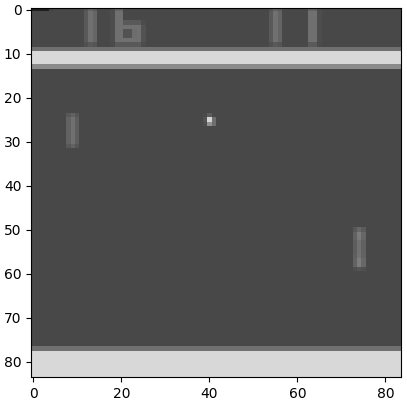
\includegraphics[width=\linewidth]{Pong/State_original}
		\caption{The original observation, i.e. the input for the PCA transformation.}
		\label{fig:pca-original-pong} 
	\end{subfigure}\hfill
	\begin{subfigure}[b]{0.3\textwidth}
		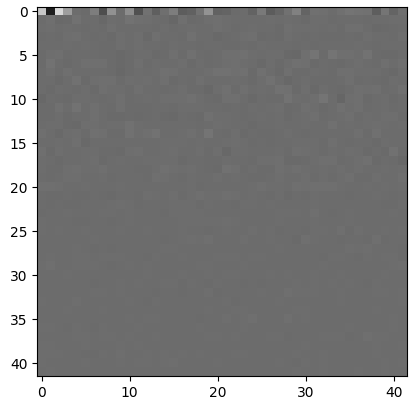
\includegraphics[width=\linewidth]{Pong/State_pca}
		\caption{The latent representation given by the PCA transformation}
		\label{fig:pca-latent-pong}
	\end{subfigure}
	\caption{Latent representation of a state observation using PCA in Pong.}
	\label{fig:pca-state-pong}
\end{figure}

\paragraph{Pre-trained autoencoder agent: slightly worse than the baseline agent}
Unlike in the Starcraft II environment, the pre-trained autoencoder agent performs slightly worse than the baseline agent in Pong. Though getting similar scores for most episodes, the autoencoder agent is initially less consistent, which is shown by occasional low scoring episodes up until episode $350$. However, the agent still converges to a rather decent policy despite using $42 \times 42$ latent representations.

To analyse and validate the results of the autoencoder, we first show the output of the encoder, i.e. the latent representation, in figure \ref{fig:ae-output-pong-pre}. What can be seen here is a compression of the data similar to the autoencoder in Starcraft II. Each pixel in the latent representation correlates to a block of pixels of the original data. Thus, a pixel's value in the latent representation will reflect the values of a block of pixels in the original image, and therewith compress the data to a lower dimensional space. 

\begin{figure}[h]
	\centering
	\begin{subfigure}[b]{0.40\textwidth}
		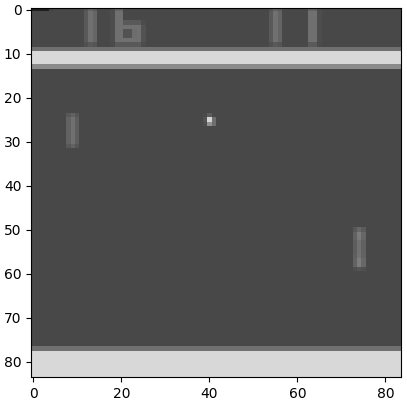
\includegraphics[width=\linewidth]{Pong/State_original}
		\caption{The original observation frame, i.e. the input for the autoencoder.}
	\end{subfigure}\hfill
	\begin{subfigure}[b]{0.40\textwidth}
		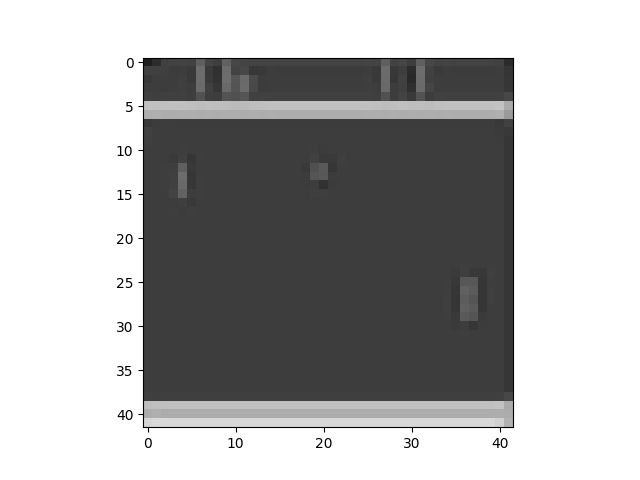
\includegraphics[width=\linewidth]{Pong/State_ae1_output}
		\caption{The output of the encoder of the pre-trained autoencoder.}
		\medskip
	\end{subfigure}
	\caption{Latent representation the pre-trained autoencoder for an observation frame in Pong.}
	\label{fig:ae-output-pong-pre}
\end{figure}

This can explain why the agent learns a sub-optimal policy: the lower dimensional space creates slight imprecisions with regards to the exact locations of the ball and the paddles. In the Starcraft II environment this did not create problems since the beacon spans a relatively large space. However, in Pong the ball is only four pixels large and its precise location relative to the paddle is very important for deciding where to move the paddle to. As we will see in later analyses given here, more precise latent representation result in better RL agent scores.

Like in the Starcraft II discussion, we now also give the correlation matrix, following the same process as before, visualised in figure \ref{fig:ae-corr-process}. We create a correlation matrix based on $40.000$ frames between the original $84 \times 84$ features and the $42 \times 42$ latent features given by the autoencoder's encoder. The resulting matrix is given in figure \ref{fig:ae-corr-pong}. Again, to visualise this better, we show the correlation matrix of a single latent feature with the original features. We do this by taking the values of a single column corresponding to a latent feature from the correlation matrix, and then reshape this to the $84 \times 84$ grid.

We show this for two latent features. The first is a latent feature that is centered in the latent grid, shown in figure \ref{fig:ae-latent-feature-pong}. What can be seen in its correlation matrix in figure \ref{fig:ae-latent-feature-corr-matrix-pong} is that there is high correlation of the latent feature with a square of original features in the same relative space. This could represent the ball in Pong, as that is the only object moving through this part of the screen. When we relate this to the correlation results from Starcraft II, we can see a similar pattern: the latent features correlate with a figure surrounding the same relative space in the original features. In Starcraft II, this took the form of the beacon: an octagon. This time, it takes the form of the ball.

Interesting results also come from a different latent feature shown in figure \ref{fig:ae-latent-feature-pong2}. This is placed in the relative space of the right paddle in the original observation. The correlation matrix shown in figure \ref{fig:ae-latent-feature-corr-matrix-pong2} shows a high correlation in the shape of the paddle in the same relative space.

\begin{figure}[h]
	\centering
	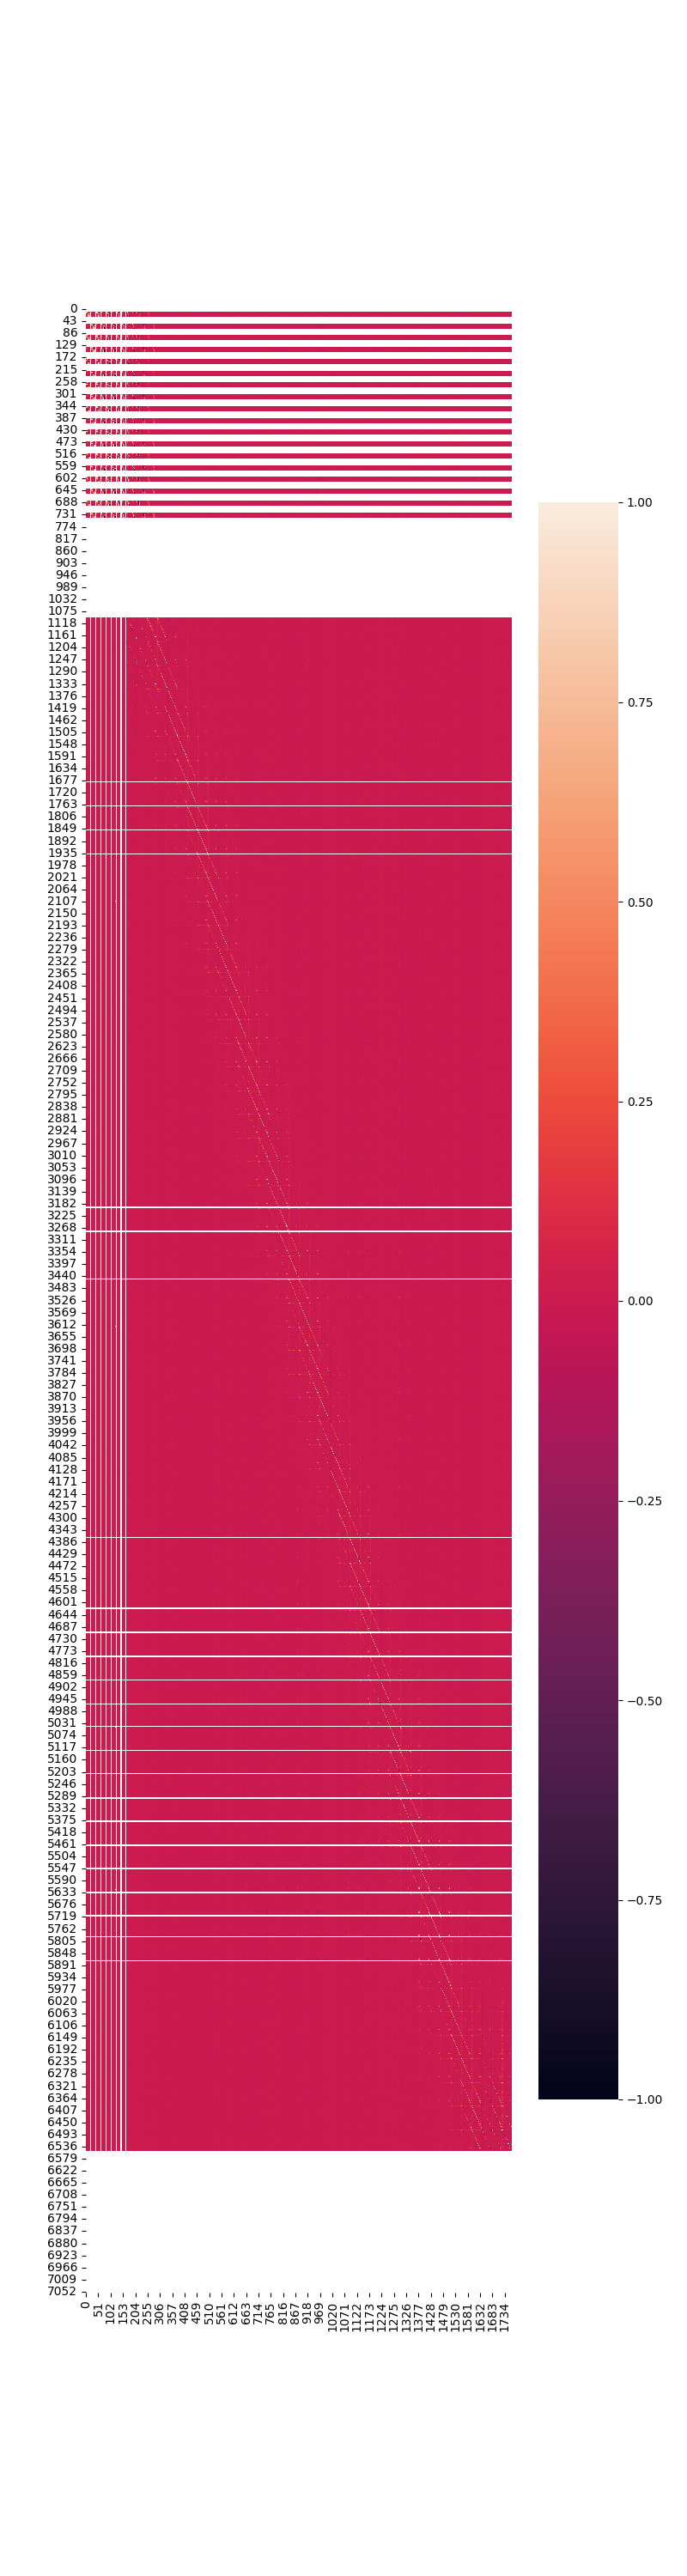
\includegraphics[height=0.90\textheight]{Pong/corr_matrix_reduced}
	\caption{Correlation matrix for the autoencoder used in the pre-trained autoencoder agent in Pong, based on $40.000$ state observations. The x-axis contains the features of the reduced state observations, and the y-axis contains the features of the original observations. Certain parts are zoomed into, revealing the correlation pattern.}
	\label{fig:ae-corr-pong}
\end{figure}

\begin{figure}[h]
	\centering
	\begin{subfigure}[b]{0.2\textwidth}
		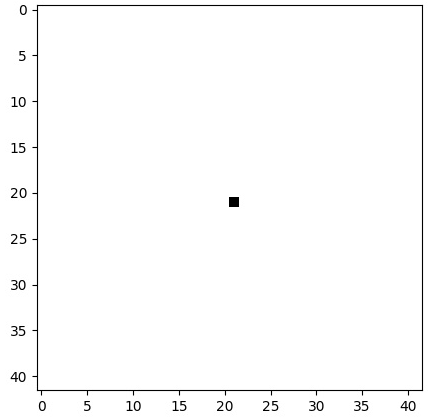
\includegraphics[width=\linewidth]{Pong/grid_latent_feature_904}
		\caption{The latent feature that was used: at index $903$ of flattened grid data.}
		\label{fig:ae-latent-feature-pong} 
	\end{subfigure}\hfill
	\begin{subfigure}[b]{0.75\textwidth}
		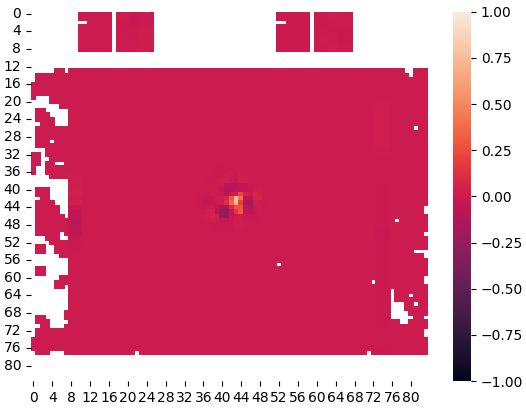
\includegraphics[width=\linewidth]{Pong/corr_matrix_latent_feature_904}
		\caption{The correlation matrix for latent feature $904$ with the original features.}
		\label{fig:ae-latent-feature-corr-matrix-pong}
	\end{subfigure}
	\caption{The correlation matrix for latent feature $904$ with the original features.}
	\label{fig:latent-feature-corr-pong}
\end{figure}

\begin{figure}[h]
	\centering
	\begin{subfigure}[b]{0.2\textwidth}
		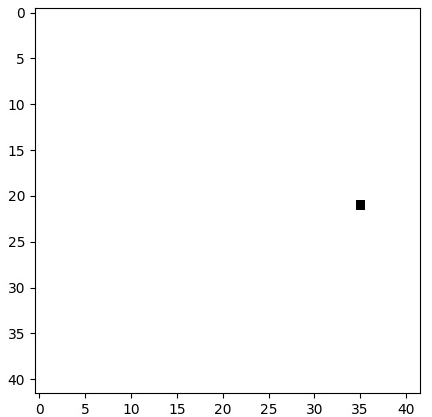
\includegraphics[width=\linewidth]{Pong/grid_latent_feature_918}
		\caption{The latent feature that was used: at index $917$ of flattened grid data.}
		\label{fig:ae-latent-feature-pong2} 
	\end{subfigure}\hfill
	\begin{subfigure}[b]{0.75\textwidth}
		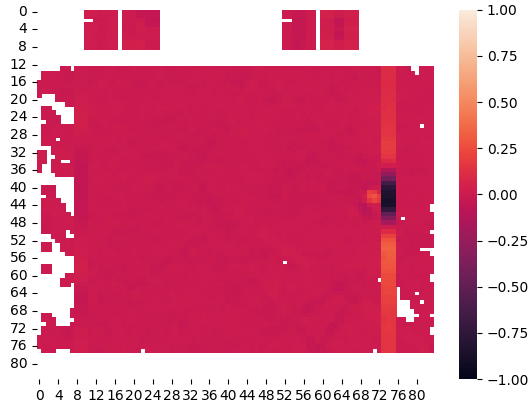
\includegraphics[width=\linewidth]{Pong/corr_matrix_latent_feature_918}
		\caption{The correlation matrix for latent feature $918$ with the original features.}
		\label{fig:ae-latent-feature-corr-matrix-pong2}
	\end{subfigure}
	\caption{The correlation matrix for latent feature $918$ with the original features.}
	\label{fig:latent-feature-corr-pong2}
\end{figure}

To further validate the autoencoder agent's results, we trained three other autoencoders on a lower number of frames; the autoencoder used so far will be named \emph{autoencoder 1} and the three remaining autoencoders will be named \emph{autoencoder 2}, \emph{autoencoder 3}, and \emph{autoencoder 4}, where autoencoder 4 is trained on the fewest number of frames. These three additional autoencoders are used in two ways. First, we take the trained autoencoder agent (i.e. trained on the original autoencoder: autoencoder 1) and replace autoencoder 1 with autoencoders 2, 3 and 4. This way we can see how much the agent depends on the specific encoding of the autoencoder it was trained on. Secondly, we will train three additional autoencoder agents on the other two pre-trained autoencoders. This way we can compare the effect of using a less accurate autoencoder on the RL agent.

The losses of the autoencoders (computed by the difference between the input image and the latent representation, as explained in section \ref{pl-ae}) during training can be seen in figure \ref{fig:ae-loss-pong}. An untrained autoencoder has a loss of roughly $1500$. Autoencoder 1 was trained on $925.000$ frames and ended in a loss of $0.3$. Autoencoder 2 was trained on $340.000$ frames and ended in a loss of $0.9$. Autoencoder 3 was trained on $25.000$ frames and ended in a loss of $30.7$. Finally, autoencoder 4 was trained on $10.000$ frames and ended in a loss of $86.2$. The full training progress for autoencoder 1 is not shown, in favor of giving a clearer view on the training of the additional three autoencoders. However, this autoencoder is trained on the same initial frames, and hence it trains further where autoencoder 2 left off.

\begin{figure}[h]
    \centering
   	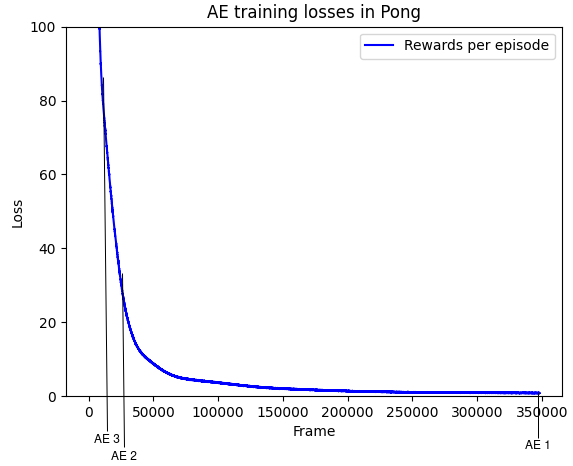
\includegraphics[width=0.6\textwidth]{Pong/AE_losses_pong}
    	\caption{Losses per frame for training three autoencoders in Pong. Autoencoder 1 trained on $925.000$ frames to a loss of $0.3$, autoencoder 2 trained on $340.000$ frames to a loss of $0.9$, autoencoder 3 trained on $25.000$ frames to a loss of $30.7$ and autoencoder 4 trained on $10.000$ frames to a loss of $86.2$.}
    	\label{fig:ae-loss-pong}
\end{figure}

The effect of this difference in loss and number of training frames, is shown in figure \ref{fig:ae-output-pong}. Here we can see the latent representation for the three new autoencoders. In other words, they show the output of the encoder, for a given frame. It can be clearly seen that, although each latent representation is similar, the better autoencoder gives a more precise representation of the original image. Thus, it retains more spatial information and should result in a better autoencoder agent.

\begin{figure}[h]
	\centering
	\begin{subfigure}[b]{0.40\textwidth}
		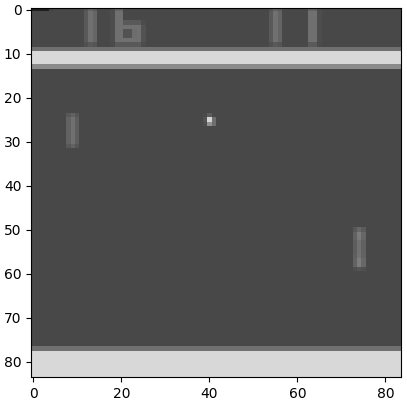
\includegraphics[width=\linewidth]{Pong/State_original}
		\caption{The original observation frame, i.e. the input for the autoencoder.}
		\label{fig:ae-state-original-pong} 
	\end{subfigure}\hfill
	\begin{subfigure}[b]{0.40\textwidth}
		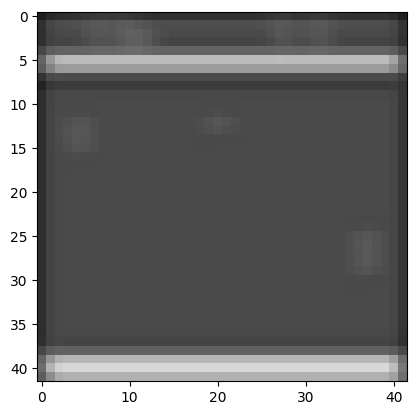
\includegraphics[width=\linewidth]{Pong/State_ae2_output}
		\caption{The output of the encoder of autoencoder 2.}
		\medskip
		\label{fig:ae1-state-pong}
	\end{subfigure}
	\begin{subfigure}[b]{0.4\textwidth}
		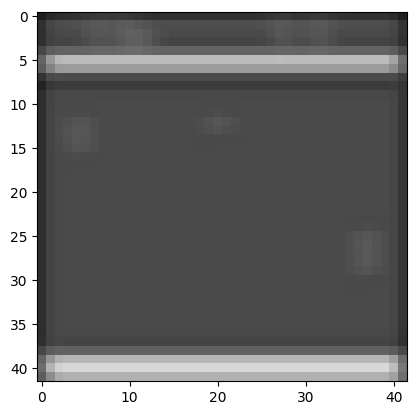
\includegraphics[width=\linewidth]{Pong/State_ae3_output}
		\caption{The output of the encoder of autoencoder 3.}
		\label{fig:ae2-state-pong}
	\end{subfigure}\hfill
	\begin{subfigure}[b]{0.4\textwidth}
		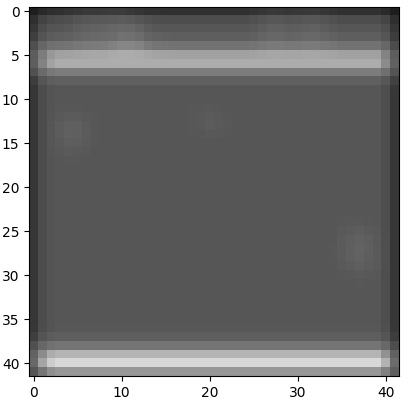
\includegraphics[width=\linewidth]{Pong/State_ae4_output}
		\caption{The output of the encoder of autoencoder 4.}
		\label{fig:ae3-state-pong}
	\end{subfigure}
	\caption{Latent representations of three different autoencoders for an observation frame in Pong. The more frames the autoencoder was trained, the more precise its latent representation is; from autoencoder 2 to autoencoder 4 the latent representations are increasingly less accurate.}
	\label{fig:ae-output-pong}
\end{figure}

The first way we use these additional autoencoders to analyse the pre-trained autoencoder agent, is by taking the RL agent trained on autoencoder 1 and replacing the autoencoder with each of the other three. This way we can see how much the RL agent's training depends on the specific encoding it was trained on. The results given in figure \ref{fig:ae-evals} show that the RL agents depends a lot on the specific autoencoder it was trained on. Only  when using autoencoder 2, trained to a loss of 0.9, was the RL agent able to get scores higher than $-21$, but it still scored only around $-7$. As we will see next, an RL agent trained on this autoencoder can actually reach a policy scoring around $15$.

\begin{figure}[h]
	\centering
	\begin{subfigure}[b]{0.40\textwidth}
		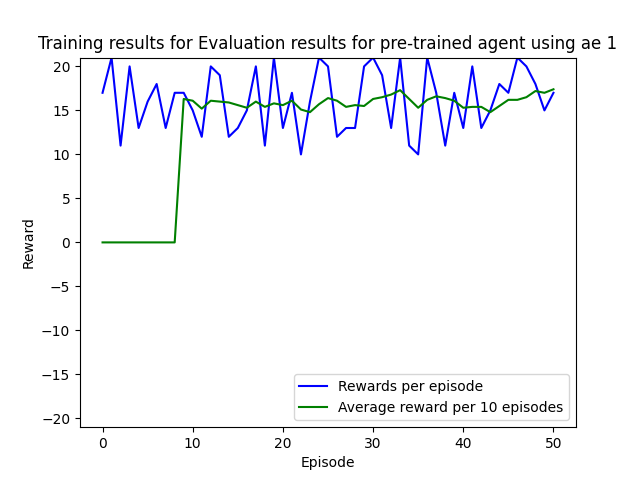
\includegraphics[width=\linewidth]{Pong/Results_eval_ae1}
		\caption{Evaluation results using autoencoder 1.}
	\end{subfigure}\hfill
	\begin{subfigure}[b]{0.40\textwidth}
		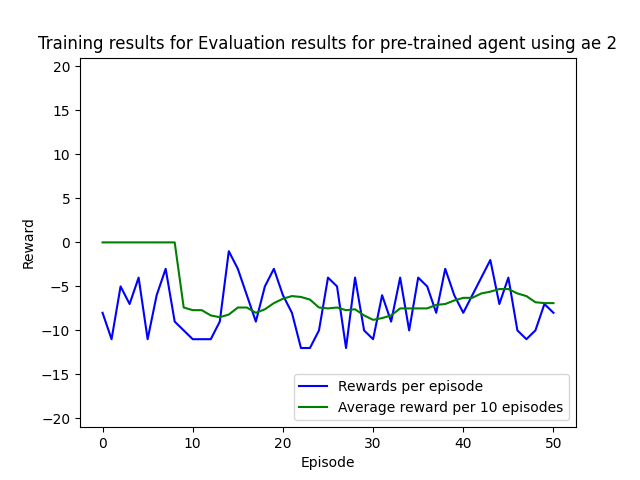
\includegraphics[width=\linewidth]{Pong/Results_eval_ae2}
		\caption{Evaluation results using autoencoder 2.}
		\medskip
	\end{subfigure}
	\begin{subfigure}[b]{0.4\textwidth}
		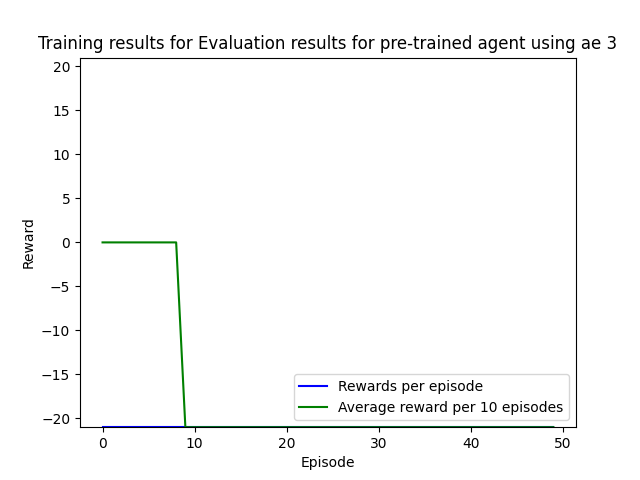
\includegraphics[width=\linewidth]{Pong/Results_eval_ae3}
		\caption{Evaluation results using autoencoder 3.}
	\end{subfigure}\hfill
	\begin{subfigure}[b]{0.4\textwidth}
		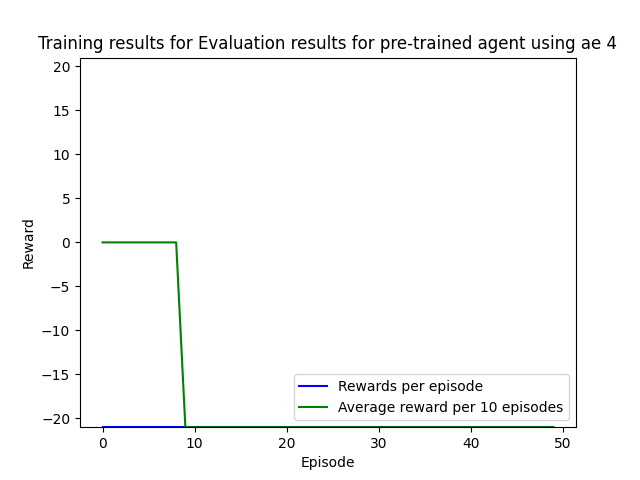
\includegraphics[width=\linewidth]{Pong/Results_eval_ae4}
		\caption{Evaluation results using autoencoder 4.}
	\end{subfigure}
	\caption{Results for evaluating the pre-trained autoencoder agent while replacing its autoencoder.}
	\label{fig:ae-evals}
\end{figure}

The second use of the additional autoencoders is to show the effect on an RL agent when using less accurate latent representations. We do this by training different RL agents (from scratch) on these additional autoencoders. The results can be seen in figure \ref{fig:ae-results-pong}: the better the autoencoder being used by the RL agent, the better the agent trains. We have already looked at the results for autoencoder 1, in figure \ref{fig:ae1-results-pong}, and how it compared to the baseline agent. We can see in figure \ref{fig:ae2-results-pong} that using autoencoder 2, results in a slightly worse RL agent. Most notably it is less consistent: it keeps having episodes with very low scores, which can also be seen by the oscillating average score. However, its average score is still fairy good, oscillating around $15$. The second additional autoencoder, autoencoder 3, scores a lot worse, shown in figure \ref{fig:ae3-results-pong}. It takes more episodes to converge compared to the agent using autoencoder 1 ($180$ and $250$ episodes respectively) and converges to a less optimal policy. In particular, it is a lot less consistent, often scoring even below $0$ (thus losing the Pong game). The agent using autoencoder 4, shown in figure \ref{fig:ae4-results-pong} performs even worse than this. It takes about $300$ episodes before it starts getting to a policy that is better than a random agent, and after $400$ gets to a very inconsistent policy: it both has episodes of $21$ and of $-21$. Its results are very similar to that of the PCA agent, which lost all spatial information in its latent representation. Thus, it is clearly seen that the less accurate the autoencoder, the less the RL agent is able to train on its latent representation, thereby showing the importance of a well trained autoencoder when used for state-space dimensionality reduction.


\begin{figure}[h]
	\centering
	\begin{subfigure}[b]{0.49\textwidth}
		\includegraphics[width=1\linewidth]{Pong/Pretrained_autoencoder_agent_results}
		\caption{Training results for RL agent using pre-trained autoencoder 1 in Pong.}
		\label{fig:ae1-results-pong}
	\end{subfigure}
	\begin{subfigure}[b]{0.49\textwidth}
		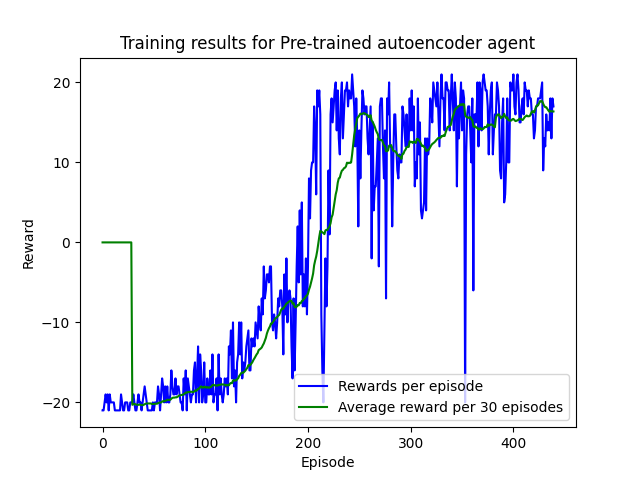
\includegraphics[width=1\linewidth]{Pong/Pretrained_autoencoder_2_agent_results}
		\caption{Training results for RL agent using pre-trained autoencoder 2 in Pong.}
		\label{fig:ae2-results-pong}
	\medskip
	\end{subfigure}
	\begin{subfigure}[b]{0.49\textwidth}
		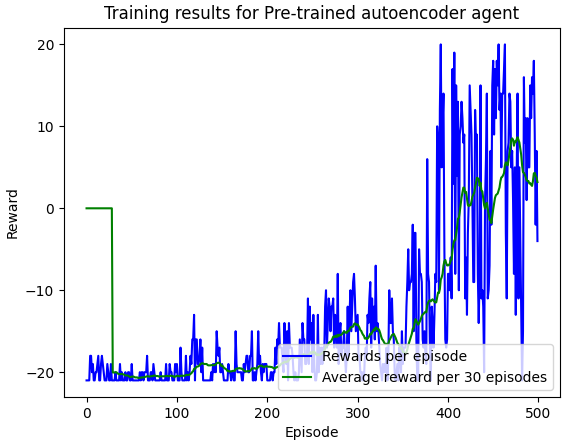
\includegraphics[width=1\linewidth]{Pong/Pretrained_autoencoder_3_agent_results}
		\caption{Training results for RL agent using pre-trained autoencoder 3 in Pong.}
		\label{fig:ae3-results-pong}
	\end{subfigure}
	\begin{subfigure}[b]{0.49\textwidth}
		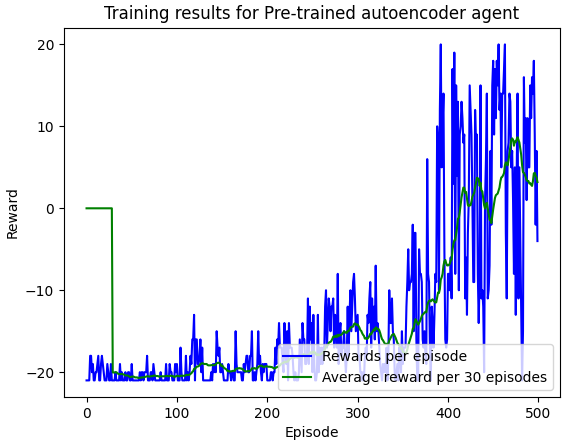
\includegraphics[width=1\linewidth]{Pong/Pretrained_autoencoder_4_agent_results}
		\caption{Training results for RL agent using pre-trained autoencoder 4 in Pong.}
		\label{fig:ae4-results-pong}
	\end{subfigure}
	\caption{Training results for three different pre-trained autoencoder agents in Pong. Autoencoders 1 to 4 are trained to an increasing loss value (i.e. decreasing number of frames). Training to lower losses results in better latent representations, which result in better RL agents.}
	\label{fig:ae-results-pong}
\end{figure}

\clearpage
\paragraph{Online trained autoencoder agent: equaling the pre-trained autoencoder agent's policy}
Lastly we have the online trained autoencoder agent. Interestingly, this agent converges to a policy similar to the pre-trained autoencoder agent.

These results can both be explained by the way the autoencoder is trained. Because the autoencoder is trained simultaneously with the RL agent, the RL agent initially trains on bad latent representations, given by a barely trained encoder. Thus, initially the RL agent is unable to train well. Furthermore, during the initial stages of training the autoencoder, its latent representations will change significantly, meaning the RL agent will receive very differing latent representations for the same (or similar) state observations. This results in the RL agent needing more episodes to converge than the baseline agent.

Its converging policy being similar to the pre-trained agent, can also be explained by the way the autoencoder is trained. Because we are training on $500$ episodes, the online trained autoencoder is trained on a similar number of frames as the pre-trained autoencoder. Consequently, the training loss of the autoencoder component is eventually similar to that of the pre-trained autoencoder. Thus, it is able to give a precise latent representation, which as we just saw in the analysis of the pre-trained autoencoder agent, results in better RL training results.

Interestingly, the output of these two autoencoders are only slightly, barely visibly different. The pre-trained autoencoder trained to a loss of $0.2$ for reconstructing the original observation from its latent representation. The online trained autoencoder reaches this same loss value around episode $220$. It finally ends at a loss of $0.45$ (tested on the same data set as the pre-trained autoencoder). The output of the encoders of both autoencoders can be seen in figure \ref{fig:online-ae-output-pong}.

\begin{figure}[h]
	\centering
	\begin{subfigure}[b]{0.45\textwidth}
		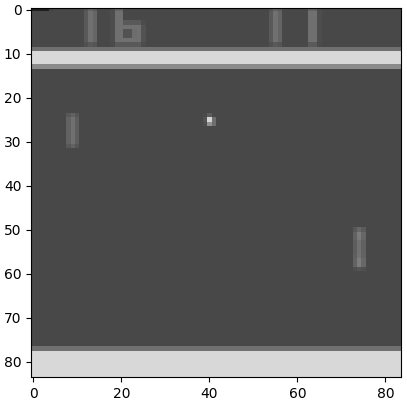
\includegraphics[width=1\linewidth]{Pong/State_original}
		\caption{The original observation frame, i.e. the input for the autoencoder.}
	\end{subfigure}\hfill
	\begin{subfigure}[b]{0.45\textwidth}
		\includegraphics[width=1\linewidth]{Pong/State_ae1_output}
		\caption{The output of the encoder of the pre-trained autoencoder.}
	\end{subfigure}\medskip
	\begin{subfigure}[b]{0.45\textwidth}
		\includegraphics[width=1\linewidth]{Pong/State_onlineae_output}
		\caption{The output of the encoder of the online trained autoencoder.}
	\end{subfigure}
	\caption{Latent representations of the pre-trained autoencoder and online trained autoencoder for an observation frame in Pong.}
	\label{fig:online-ae-output-pong}
\end{figure}

\clearpage
\subsection{Results discussion}\label{research-discussion}
As we have seen in the results from our experiments in Starcraft II and OpenAI Pong, the effect of state-space dimensionality reduction on reinforcement learning depends on the technique and environment used. 

Both PCA and DeepMDP did not work well in both our environments and resulted in RL agents having difficulty training, or not training at all. For PCA, this was the result of losing spatial information in its latent representation. Curran et al. showed that it is indeed possible to get an RL agent to learn on the latent space of PCA \cite{mario}. This they did on non-spatial (linear) observations. Thus, the effectiveness of using PCA for state-space dimensionality reduction depends on whether it uses spatial or linear observations.

Although the DeepMDP agent was able to get to a decent policy in our Starcraft II environment, it had difficulty with balancing the different loss calculations. This is also mentioned in the paper introducing the DeepMDP architecture \cite{deepmdp}. This balancing issue resulted in network updates that lowered one loss calculation, but raised another. Hence, the policy network was not able to train well. Furthermore, the DeepMDP took a lot more time to train per episode than all other agents, due to an additional network being used.

The use of the autoencoder was the most promising method for state-space dimensionality reduction in reinforcement learning. In both the Starcraft II and the Pong environment, the autoencoder projected the data to a space that is 4 times lower than the original state-space, while reaching an optimal RL policy. However, some spatial information might get lost in its compression. For Starcraft II this was not a problem due to the beacon being fairly large. Here, the pre-trained autoencoder agent was able to train quicker to a better policy than the baseline agent. This is a result of the policy network being trained on smaller input, having to consider fewer states. However, in Pong the location of the ball and the paddle need to be precise in order to get an optimal agent. The imprecise spatial-information of the pre-trained autoencoder therefore resulted in an agent that performed slightly worse than the baseline agent. This was corroborated  by training multiple RL agents on autoencoders trained to different losses, i.e. with latent representations differing in accuracy. The more accurate the latent representation was, the better the RL agent was able to train. The online trained autoencoder agents generally reach similar policies as the pre-trained autoencoder agents. However, due to having to train the autoencoder simultaneously with the RL agent, it tends to take more episodes to converge. 

The effect of the accuracy of the latent representation on the RL agent, also shows the limits of using an autoencoder. When there is a lot of detailed spatial information, some of this might get lost in the latent representation of the autoencoder. Thus, using an autoencoder for state-space dimensionality reduction in such environments could lead to sub-optimal policies.

As for training times, the use of a PCA component or autoencoder adds a very little, negligible amount of time to train the RL agent. Thus the baseline agent, PCA agent and pre-trained autoencoder agent all have similar training times. Pre-training the PCA component and autoencoder took relatively little time as well, resulting in an increase in training time for the online trained autoencoder agent of $3.3\%$ and $4.7\%$ for Starcraft II and Pong respectively. The DeepMDP agent however takes a lot longer to train; in Starcraft II, each episode took around $2.5$ minutes to train, in contrast with the $\sim3$ seconds per episode for the baseline agent.